\chapter{Example Graphs for Validation}
\label{chap:validation_examples}

In this chapter, we provide test graphs containing the expected results for
BFS (\autoref{fig:bfs_example}),
CDLP (\autoref{fig:cdlp_example}),
LCC (\autoref{fig:lcc_example}),
SSSP (\autoref{fig:sssp_example}),
WCC (\autoref{fig:wcc_example}),
and a common example for all six algorithms (\autoref{fig:common_example}).
The PageRank test graphs (\texttt{test-pr-directed} and \texttt{test-pr-undirected}) are provided in the data sets but not displayed here due to their relatively large sizes (50~nodes).

\newcommand{\examplescale}{0.48}

\begin{figure}[h]
	\centering
	\begin{subfigure}{0.496\textwidth}
		\centering
		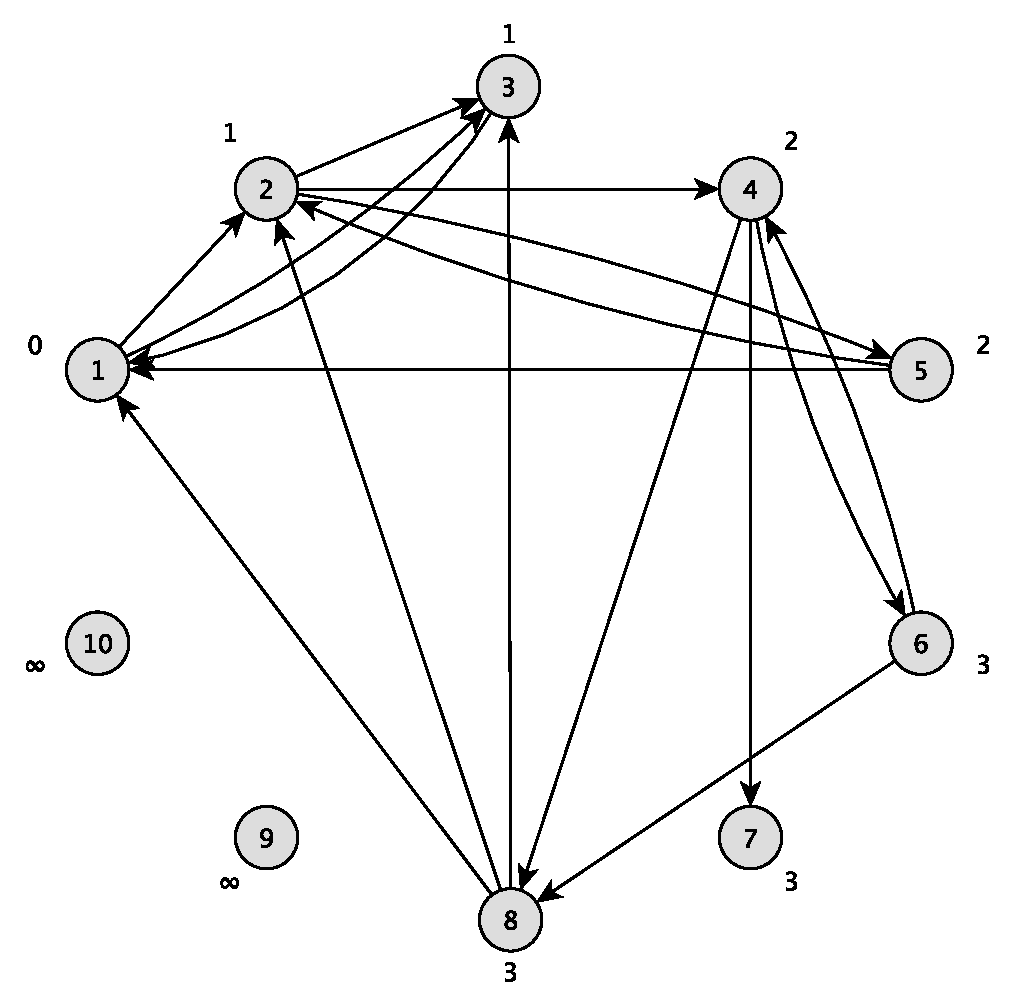
\includegraphics[scale=\examplescale]{figures/examples/bfs-dir.pdf}
		\caption{Directed (\texttt{text-bfs-directed})}
	\end{subfigure}
	\begin{subfigure}{0.496\textwidth}
		\centering
		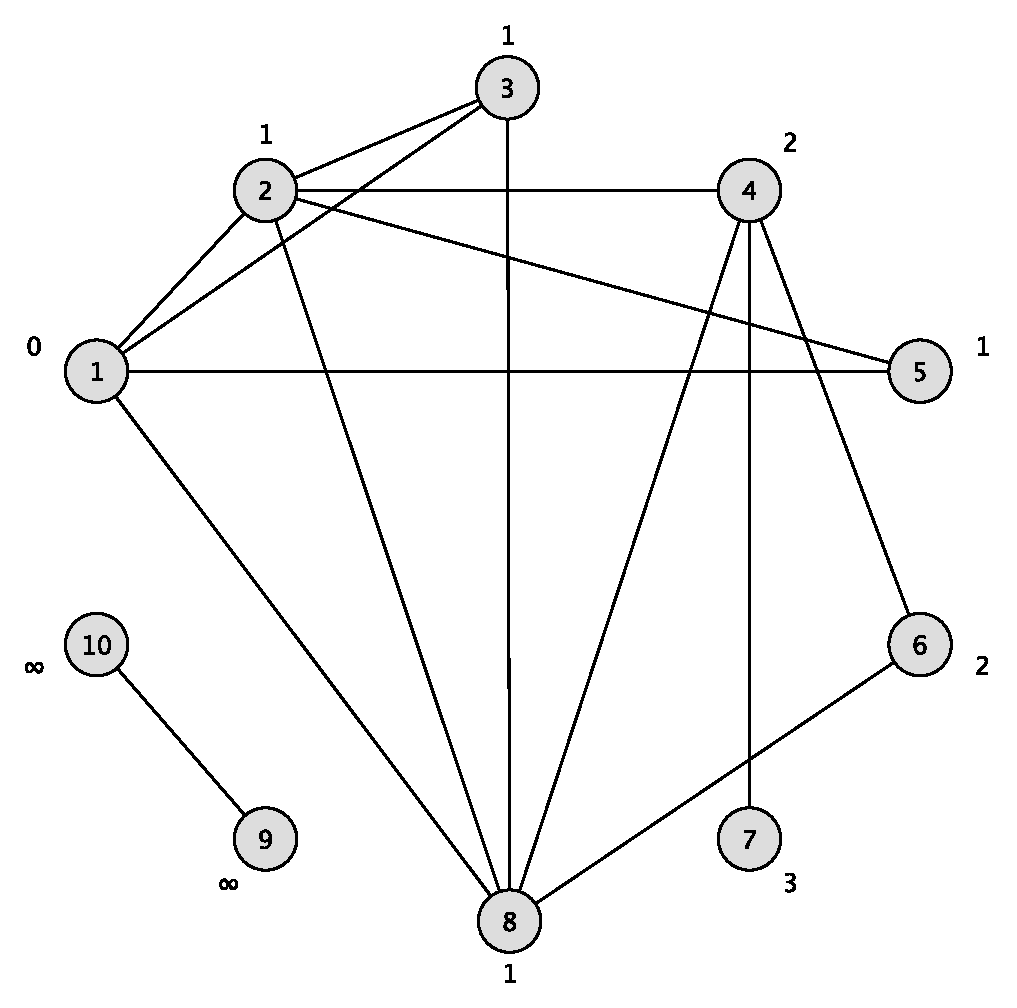
\includegraphics[scale=\examplescale]{figures/examples/bfs-undir.pdf}
		\caption{Undirected (\texttt{text-bfs-undirected})}
	\end{subfigure}
	\caption{Test graphs for BFS. Source vertex: 1.}
	\label{fig:bfs_example}
\end{figure}

\begin{figure}[h]
	\centering
	\begin{subfigure}{0.496\textwidth}
		\centering
		\includegraphics[scale=\examplescale]{figures/examples/cdlp-dir.pdf}
		\caption{Directed (\texttt{text-cdlp-directed})}
	\end{subfigure}
	\begin{subfigure}{0.496\textwidth}
		\centering
		\includegraphics[scale=\examplescale]{figures/examples/cdlp-undir.pdf}
		\caption{Undirected (\texttt{text-cdlp-undirected})}
	\end{subfigure}
	\caption{Test graphs for CDLP. Maximum number of iterations: 5.}
	\label{fig:cdlp_example}
\end{figure}

\begin{figure}[h]
	\centering
	\begin{subfigure}{0.496\textwidth}
		\centering
		\includegraphics[scale=\examplescale]{figures/examples/lcc-dir.pdf}
		\caption{Directed (\texttt{text-lcc-directed})}
	\end{subfigure}
	\begin{subfigure}{0.496\textwidth}
		\centering
		\includegraphics[scale=\examplescale]{figures/examples/lcc-undir.pdf}
		\caption{Undirected (\texttt{text-lcc-undirected})}
	\end{subfigure}
	\caption{Test graphs for LCC.}
	\label{fig:lcc_example}
\end{figure}

\begin{figure}[h]
	\centering
	\includegraphics[scale=\examplescale]{figures/examples/lcc-dir-example-detailed.pdf}
	\caption{Detailed example of LCC values on a directed graph. Each graph represents a projected subgraph with a selected vertex (colored in gray) and its neighbors.
		Thick edges (denote the edges between the neighbors, while thin edges denote the edges from the vertex to its neighbors.
		As discussed in \autoref{sec:lcc}, the set of neighbors is determined without taking directions into account, but each neighbor is only counted once. However, directions are enforced when determining the number of edges (thick) between neighbors.
		Note that vertices 6, 7, 9, and 10 have an LCC value of 0.00 and are therefore omitted from the visualization.}
	\label{fig:lcc_dir_example_detailed}
\end{figure}

\begin{figure}[h]
	\centering
	\begin{subfigure}{0.496\textwidth}
		\centering
		\includegraphics[scale=\examplescale]{figures/examples/sssp-dir.pdf}
		\caption{Directed (\texttt{text-sssp-directed})}
	\end{subfigure}
	\begin{subfigure}{0.496\textwidth}
		\centering
		\includegraphics[scale=\examplescale]{figures/examples/sssp-undir.pdf}
		\caption{Undirected (\texttt{text-sssp-undirected})}
	\end{subfigure}
	\caption{Test graphs for SSSP. Source vertex: 1.}
	\label{fig:sssp_example}
\end{figure}

\begin{figure}[h]
	\centering
	\begin{subfigure}[t]{0.496\textwidth}
		\centering
		\includegraphics[scale=\examplescale]{figures/examples/wcc-dir.pdf}
		\caption{Directed (\texttt{text-wcc-directed}). Note that due to the semantics of the WCC algorithm, the direction of the edges is not taken into account, i.e., they are treated as undirected edges.}
	\end{subfigure}
	\begin{subfigure}[t]{0.496\textwidth}
		\centering
		\includegraphics[scale=\examplescale]{figures/examples/wcc-undir.pdf}
		\caption{Undirected (\texttt{text-wcc-undirected})}
	\end{subfigure}
	\caption{Test graphs for WCC. Remark: there are 8 nodes indexed between 1 and 9 but number 5 is not assigned to any of the nodes.}
	\label{fig:wcc_example}
\end{figure}

\begin{figure}[h]
	\centering
	\begin{subfigure}{\textwidth}
		\centering
		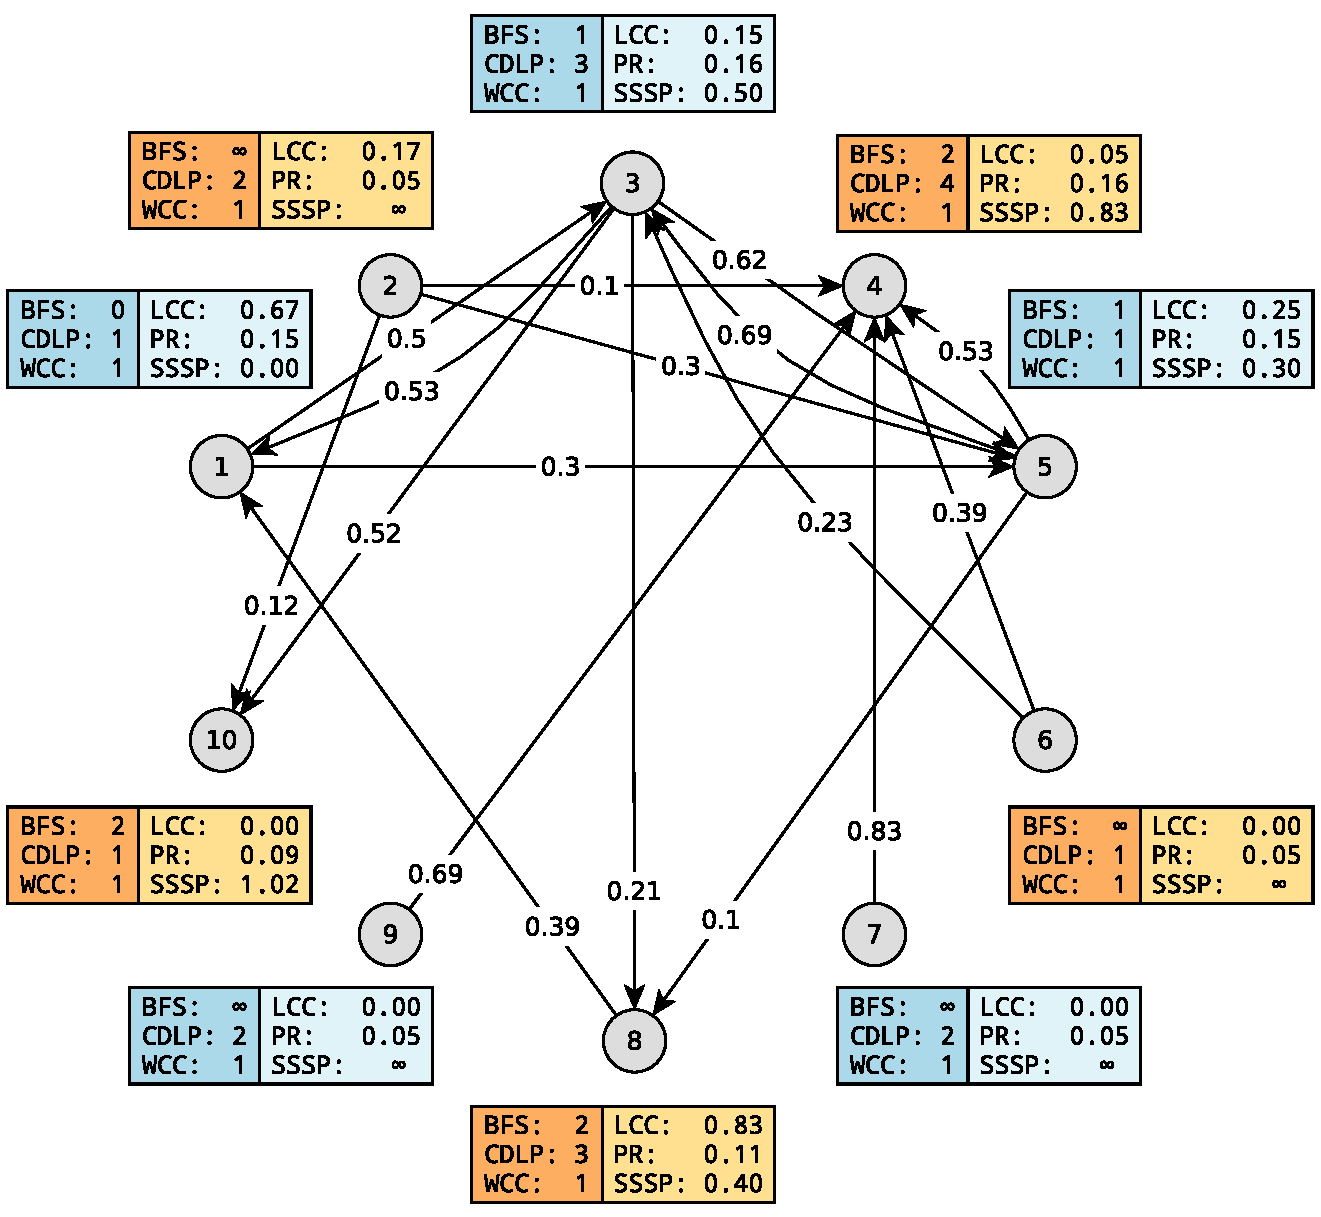
\includegraphics[scale=\examplescale]{figures/examples/common-dir.pdf}
		\caption{Directed (\texttt{example-directed}).
			Algorithm parameters --
			BFS: source vertex = 1.
			CDLP: maximum number of iterations = 2.
			PR: $d = 0.85$, maximum number of iterations = 2.
			SSSP: source vertex = 1.}
	\end{subfigure}
	\begin{subfigure}{\textwidth}
		\centering
		\includegraphics[scale=\examplescale]{figures/examples/common-undir.pdf}
		\caption{Undirected (\texttt{example-undirected}).
			Algorithm parameters --
			BFS: source vertex = 2.
			CDLP: maximum number of iterations = 2.
			PR: $d = 0.85$, maximum number of iterations = 2.
			SSSP: source vertex = 2.}
	\end{subfigure}
	\caption{Common examples for the six core graph algorithms.}
	\label{fig:common_example}
\end{figure}
